\documentclass{beamer}

\makeatletter
\def\input@path{{usyd-beamer-theme/}}
\makeatother

\usepackage{babel}
\babelprovide[main, import]{croatian}

\graphicspath{{usyd-beamer-theme/}}

\mode<presentation>
{%
    \usetheme{usyd}
}

% Override title page background: remove image and USYD branding
\setbeamertemplate{background}{%
  \begin{tikzpicture}
    \useasboundingbox (0,0) rectangle(\the\paperwidth, \the\paperheight);
    \ifnum\thepage=1\relax%
      \fill[color=usydred] (0,0) rectangle (\the\paperwidth, \the\paperheight);
    \else
      \fill[color=usydwhite] (0,0) rectangle (\the\paperwidth, \the\paperheight);
    \fi
  \end{tikzpicture}
}

% Remove logo from title page
\setbeamertemplate{logo titlepage}{}
\setbeamertemplate{affiliationlogo titlepage}{}

% Remove "University of Sydney" from footline
\setbeamertemplate{footline}{}

% Override title page to include institute
\defbeamertemplate*{title page}{custom}[1][]
{%
    \vfill
    \begin{beamercolorbox}[sep=0pt, #1]{title}
        \usebeamerfont{title}\inserttitle\par%
        \ifx\insertsubtitle\@empty\else%
          \vskip0.25em%
          {\usebeamerfont{subtitle}\usebeamercolor[fg]{subtitle}\insertsubtitle\par}%
        \fi%
    \end{beamercolorbox}\vskip1.5em
    \begin{beamercolorbox}[sep=0pt, #1]{author}
        \usebeamerfont{author}\insertauthor%
    \end{beamercolorbox}\vskip1em
    \begin{beamercolorbox}[sep=0pt, #1]{institute}
        \usebeamerfont{institute}\insertinstitute%
    \end{beamercolorbox}\vskip1em
    \begin{beamercolorbox}[sep=0pt, #1]{date}
        \usebeamerfont{date}\insertdate%
    \end{beamercolorbox}
    \vfill
}

\title{Johnsonov algoritam}
\author{Matija Njegač, Bartol Gracin}
\date{\today}
\institute{Prirodoslovno - matematički fakultet, Sveučilište u Zagrebu}

\begin{document}

\begin{frame}
    \titlepage
\end{frame}

% =============================================
% HOW TO MAKE SLIDES - quick reference:
% =============================================
%
% --- Basic slide with text ---
% \begin{frame}{Slide Title}
%   Your text here.
% \end{frame}
%
% --- Bullet points ---
% \begin{frame}{Slide Title}
%   \begin{itemize}
%     \item First point
%     \item Second point
%     \item Third point
%   \end{itemize}
% \end{frame}
%
% --- Numbered list ---
% \begin{frame}{Slide Title}
%   \begin{enumerate}
%     \item First
%     \item Second
%   \end{enumerate}
% \end{frame}
%
% --- Math formulas ---
% Inline: $a + b = c$
% Centered block: \[ a + b = c \]
%
% --- Bold / italic ---
% \textbf{bold text}  \textit{italic text}
%
% --- Image ---
% \begin{frame}{Slide Title}
%   \includegraphics[width=0.8\textwidth]{filename.png}
% \end{frame}
%
% --- Two columns ---
% \begin{frame}{Slide Title}
%   \begin{columns}
%     \begin{column}{0.5\textwidth}
%       Left side
%     \end{column}
%     \begin{column}{0.5\textwidth}
%       Right side
%     \end{column}
%   \end{columns}
% \end{frame}
%
% --- Code listing (needs \usepackage{listings} in preamble) ---
% \begin{frame}[fragile]{Slide Title}
%   \begin{lstlisting}
%     your code here
%   \end{lstlisting}
% \end{frame}
% =============================================

\begin{frame}{Johnsonov algoritam}
  Problem: naći najkraći put između svaka dva čvora u usmjerenom težinskom grafu.
  Čuli smo za Dijkstrin algoritam, ali:
  \begin{itemize}
    \item Dijkstra radi samo na grafovima gdje su težine nenegativne.
    \item Cilj: pretvoriti negativne težine u nenegativne, pa onda pokrenuti Dijkstru.
  \end{itemize}
\end{frame}

\begin{frame}{Johnsonov algoritam}
  Sastoji se od dva koraka:
  \begin{itemize}
    \item \textbf{Bellman-Ford algoritam:} pretvoriti negativne težine u nenegativne.
    \item \textbf{Dijkstrin algoritam:} naći najkraći put između svaka dva čvora u usmjerenom težinskom grafu (s
      nenegativnim težinama!)
  \end{itemize}
  \centering
  \raisebox{-.5\height}{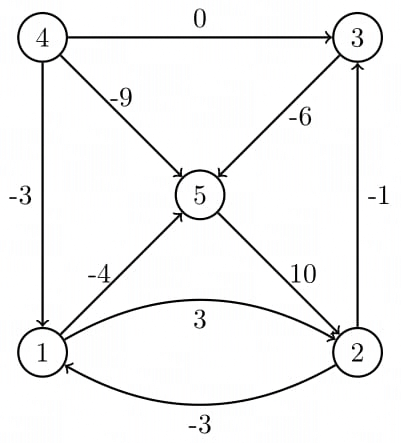
\includegraphics[width=0.4\textwidth]{slike/graf_neg.png}}%
  \raisebox{-.5\height}{
\includegraphics[width=0.1\textwidth]{slike/strelica.png}}%
  \raisebox{-.5\height}{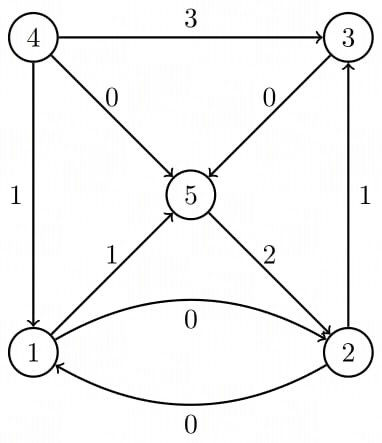
\includegraphics[width=0.4\textwidth]{slike/graf_poz.png}}
\end{frame}

\end{document}
